%!TEX root = ../thesis_polimi.tex

\chapter{System Implementation} % (fold)
\label{chap:implementation}
\start{I}{n} this chapter we discuss a few aspects concerning the implementation
of \thesystem. \thesystem is implemented in \texttt{Python}, and it uses
well known and high performance libraries for machine learning and scientific
calculus.
We discuss the system's architecture,
focusing on the process and the actors involved in the unseen domains'
classification and new threats' discovery. Moreover, we describe in deeper
detail a few core aspects of \thesystem, as the possibility of customizing
the system using an external \texttt{json} configuration file and how
we managed to address the performance challenges of the \important{Filtering Phase} leveraging the concepts of \emph{map} and \emph{reduce}.

\paragraph{Chapter Organization} The remainder of the chapter is organized in
the following fashion:
\begin{itemize}
    \item in Section~\ref{sec:system_architecture} we discuss the architecture
        of \thesystem, describing in detail the system's lifecycle and the
        actors that participate;
    \item in Section~\ref{sec:system_details} we discuss the actual implementation
        of the core parts of the system.
\end{itemize}

\newpage

\section{System Architecture} % (fold)
\label{sec:system_architecture}
\sectionstart{I}{n} this section we describe \thesystem's architecture
in a \emph{top down} fashion, first introducing the \emph{process}, i.e., how
the system analyzes the DNS data and detects botnets, and then
focusing on the \emph{actors}, the \emph{classes} and \emph{modules} that
compose \thesystem.
Before that we will provide a few technical details about the  technologies employed.

\thesystem is implemented in \texttt{Python},
version 2.7.3, and it uses \texttt{MongoDB}, version 2.4.9, as database system,
as it offers good performances. We used \texttt{Shogun}, \texttt{SciPy} and \texttt{scikit-learn} to implement the SVM with SSK classifier and the DBSCAN with SSK
clusterer, while \texttt{NumPy} offered the high-performance data structures
used in the system.

\subsection{The Process} % (fold)
\label{sub:the_process}

\thesystem needs to have two folders and a configuration file to function.
The first folder serves as a buffer where an external service (e.g., a passive DNS
monitor), sends the DNS data, which must be organized into text files where each
line is a DNS reply in \texttt{json} format.
The configuration file contains the system's settings, later to be thoroughly
explained (see Section~\ref{sub:the_configuration_file}).

After $\gamma$ time (e.g., one hour), the input files are moved to a second folder
to start the analysis process (\n{1}), while in the first folder, now emptied, the
buffering process can start over again. The DNS replies are parsed and
a list of \texttt{Domain} objects (see Section~\ref{sub:data_structures}) is created and
stored into the database (\n{2}).
This list shall later be referenced to as the \texttt{dirty\_dns} list.

Once the previous storing procedure is completed, the filtering routine can start.
The domains from the \texttt{dirty\_dns} list are loaded in memory from the
database and filtered (\n{3}) applying the
list of filters described in Section~\ref{sub:the_filtering_phase}. The resulting list
of domains, to be referred to as \texttt{cleaned\_dns}, is then stored into the
database (\n{4}).

\begin{figure}[!htp]
    \centering
    \begin{tikzpicture}[node distance=2cm]
        \node[process, label=below:Buffer Folder] (DNSSTREAM) {
\includegraphics[width=2cm]{folder.eps}};
        \node[process, right=of DNSSTREAM, , label=below:Analysis Folder] (DNSTRAFFIC) %
            {
\includegraphics[width=2cm]{folder.eps}};
        \node[process, right=of DNSTRAFFIC, label=above:\texttt{dirty\_dns}] %
        (DIRTY) {
\includegraphics[width=2cm]{database.eps}};
        \node[process, below=of DIRTY] (FILTER) %
            {
\includegraphics[width=2cm]{filter.eps}};
        \node[process, below=of FILTER, label=below:\texttt{cleaned\_dns}]%
            (CLEAN) {
\includegraphics[width=2cm]{database.eps}};
        \node[process, left=of CLEAN, , label=below:Classifier] (CLASSIFIER) %
            {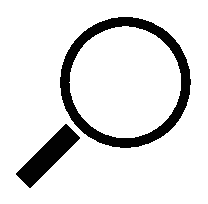
\includegraphics[width=2cm]{classifier.eps}};
        \node[process, left=of CLASSIFIER, label=below:\texttt{classified\_dns}]%
            (CLASSIFIED) {
\includegraphics[width=2cm]{database.eps}};
        \node[process, above=of CLASSIFIER, label=above:\texttt{suspicious\_ips}] %
            (SUSPICIOUS) {
\includegraphics[width=2cm]{database.eps}};
        \node[process, left=of SUSPICIOUS, , label=below:Time Detective] (TIMEDETECTIVE) %
            {
\includegraphics[width=2cm]{detective.eps}};

        \path[arrow]
            (DNSSTREAM) edge node {\n{1}} (DNSTRAFFIC)
            (DNSTRAFFIC) edge node {\n{2}} (DIRTY)
            (DIRTY) edge node {\n{3}} (FILTER)
            (FILTER) edge node {\n{4}} (CLEAN)
            (CLEAN) edge node {\n{5}} (CLASSIFIER)
            (CLASSIFIER) edge node {\n{6}} (CLASSIFIED)
            (CLASSIFIER) edge node {\n{7}} (SUSPICIOUS)
            (SUSPICIOUS) edge node {\n{8}} (TIMEDETECTIVE)
            ;
    \end{tikzpicture}
    \caption{Cerberus classification process.}
    \label{fig:cerberus_classification_process}
\end{figure}


Now the classification process can start. For each domain from the
\texttt{cleaned\_dns} list, \thesystem
first looks at the IP address and sees whether one or more clusters from the
ground truth share the same IP address (\n{5}).
In this case, a SVM is trained and a
label is assigned to the domain: All the domains for which it was possible to
assign a label are stored in a database schema called \texttt{classified\_dns}
(\n{6}).
The domains that do not share their IP address with the ground truth are not
discarded: Their IP address is stored in the \texttt{suspicious\_ips} database
schema (\n{7}). In this collection each document is composed of \emph{i)} the IP
address and \emph{ii)} the domains that resolved to that IP address throughout
time.

After $\Delta$ time, the clustering routine tries to generate new clusters to be
added to the ground truth (\n{8}). The IPs collected in the \texttt{suspicious\_ips}
schema are grouped by their respective
Autonomous System, and their lists of resolved domains are merged together. Then, for each AS, we run the DBSCAN clustering routine on
the list of domains, which produces the aforementioned new clusters of similar
domains. For instance, say we have IP $\Phi$ that resolves the domains
$\mathbb{D}(\Phi) = \{ \phi_1, \ldots, \phi_n \}$, IP $\Omega$ that
resolves the domains $\mathbb{D}(\Omega) = \{ \omega_1, \ldots, \omega_m \}$, and for the both of them the AS is $\alpha$. Then \thesystem will group
together $\Phi$ and $\Omega$, and will merge their lists of domains, obtaining
$$\mathbb{D}(\Phi, \Omega) = \{ \phi_1, \ldots, \phi_n, \omega_1, \ldots, \omega_m \}$$
that is then fed to the DBSCAN clustering routine to extract the clusters of similar malicious domains.
When this stage is terminated, \thesystem adds these clusters to its ground truth
and restarts analyzing the DNS stream, leveraging the enhanced knowledge.

Before describing the actors involved in the aforementioned process, we would
like to justify the heavy use of the database, i.e., why we chose to store the
domains at each step. The reason is to have a system \emph{failure compliant}:
If \thesystem crashes, it is possible to retrieve the results of the last completed
stage, instead of wasting time in starting the classification from the beginning.
For instance, if the system fails right after the filtering process, the list
of \texttt{cleaned\_dns} domains can be retrieved from the database and classified.
% subsection the_process (end)

\subsection{The Actors} % (fold)
\label{sub:the_actors}

\thesystem is organized into six major classes
(see Figure~\ref{fig:cerberus_overview}) of which the homonymous
\texttt{Cerberus} class is the main one, exposing the high level
functionalities of the system. It is initialized with a \texttt{config}
parameter, a \texttt{json} file that contains the variables to customize the
system at the user's needs.
\begin{figure}[!htp]
    \centering
    \begin{tikzpicture}[scale=0.85, every node/.style={transform shape}]
        \node (CERBERUS)[class] {
            \nodepart{text} Cerberus
            \nodepart{two} config
            \nodepart{three}\tabular{@{}l}%
                bootstrap() \\
                classify\_domains() \\
                execute\_daily\_routine() \\
                fetch\_dns\_cleaned\_stream() \\
                load\_configuration(path)
                \endtabular};

        \node (FILEMANAGER)[class, below=of CERBERUS] {
            \nodepart{text} FileManager
            \nodepart{two}
            \nodepart{three}\tabular{@{}l}%
            mv\_dns\_stream() \\
            clean\_folder()
            \endtabular};
        \node [above right=1.1cm and 0cm of FILEMANAGER.west] {
\includegraphics[width=.6cm]{folder.eps}};
        \node (DATAMANAGER)[class, left=of CERBERUS] {
            \nodepart{text} DataManager
            \nodepart{two}
            \nodepart{three}\tabular{@{}l}%
            classify\_dns\_cleaned\_stream() \\
            fetch\_dns\_cleaned\_stream() \\
            parse\_raw\_dns\_data()
            \endtabular};
        \node [above right= 1.3cm and 0cm of DATAMANAGER.west] (FILTERLITTLE) {
\includegraphics[width=.6cm]{filter.eps}};
        \node [right= .0cm of FILTERLITTLE]  {
\includegraphics[width=.6cm]{database.eps}};
        \node (TIMEDETECTIVE)[class,above=of CERBERUS] {
            \nodepart{text} TimeDetective
            \nodepart{two}
            \nodepart{three}\tabular{@{}l}%
            store\_suspicious\_ip\_address() \\
            cluster\_suspicious\_domains()
            \endtabular};
        \node [above right=1cm and .0cm of TIMEDETECTIVE.west]  {
\includegraphics[width=.6cm]{detective.eps}};
        \node (SVMSSKCLASSIFIER)[class,left=of TIMEDETECTIVE] {
            \nodepart{text} SVMSSKClassifier
            \nodepart{two}
            \nodepart{three}\tabular{@{}l}%
            train() \\
            classify()
            \endtabular};
        \node [above right = 1cm and 0cm of SVMSSKCLASSIFIER.west]  { %
            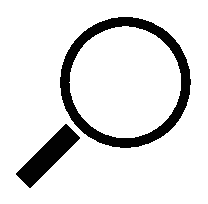
\includegraphics[width=.6cm]{classifier.eps}};
        \node (DBSCANSSKDOMAINSCLUSTERER)[class,above=of TIMEDETECTIVE] {
            \nodepart{text} DBSCANSSKDomainsClusterer
            \nodepart{two}
            \nodepart{three}\tabular{@{}l}%
            get\_clusters()
            \endtabular};

        \path[arrow]
            (CERBERUS) edge (DATAMANAGER)
            (DATAMANAGER) edge (SVMSSKCLASSIFIER)
            (TIMEDETECTIVE) edge (DBSCANSSKDOMAINSCLUSTERER)
            (CERBERUS) edge (FILEMANAGER)
            (CERBERUS) edge (TIMEDETECTIVE)
            (DATAMANAGER) edge (TIMEDETECTIVE)
        ;
    \end{tikzpicture}
    \caption{Cerberus' class diagram.}
    \label{fig:cerberus_overview}
\end{figure}
The \texttt{bootstrap()} function initializes the
system with the ground truth and it is automatically issued before the system
starts to classify the unseen domains.

The \texttt{fetch\_dns\_cleaned\_stream()} and \texttt{classify\_domains()}
subroutines are issued by the \texttt{execute\_daily\_routine()} function, which
takes care of classifying the unseen domains coming from the DNS data. They are
both executed by calls to the \texttt{DataManager} class, which offers
lower-level functionalities to \emph{i)} parse the input file of DNS data,
\emph{ii)} filter the DNS data and \emph{iii)} classify the DNS data.
While the parsing is achieved by the class itself, filtering and classification
are relayed to other modules. The \texttt{SVMSSKClassifier} takes care of
selecting the candidate clusters (those that share the IP address(es) with the
unseen domain about to be classified), train the SVM and classify the
unseen domain. The filtering process is achieved by the \texttt{stream\_filter.py}
module, described in Section~\ref{sub:the_filtering_phase}. It is not reported in
Figure~\ref{fig:cerberus_overview} as it is not a class.

The \texttt{TimeDetective} class is used by both the \texttt{DataManager} and the
\texttt{Cerberus} class. In the first case it is called the
\texttt{store\_suspicious\_ip\_address()} method, which takes care of keeping
track of the suspicious IPs and storing them in the \texttt{MongoDB} database.
In the second case, \texttt{cluster\_suspicious\_domains()} is issued,
which in turn calls the \texttt{get\_clusters()} method, which generates the
clusters of AGDs and belongs to the \texttt{DBSCANSSKDomainsClusterer} class.
Finally, the \texttt{FileManager} class handles the routines related to
filesystem calls.
% section system_architecture (end)


\section{System Details} % (fold)
\label{sec:system_details}
\sectionstart{I}{n} this section we focus on the core aspects of the
implementation of \thesystem, and provide a more detailed description. First we
present the \emph{configuration file} used to customize the system to user's needs.
Than we  briefly see the \texttt{Domain} and \texttt{DomainName} classes, used
by \thesystem to store the data throughout the analysis. Finally we tackle the
crucial aspects of the three phases of \thesystem: \important{Bootstrap},
\important{Filtering} and \important{Detection}.

\subsection{The Configuration File} % (fold)
\label{sub:the_configuration_file}
\thesystem was designed to be flexible and customizable. To this end,
we envisaged the possibility of setting a few variables via an external \texttt{json}
file. The user needs to put this file in the same folder where \thesystem is and
name it \texttt{config.json}.

\texttt{Cerberus}, the main class, is then initialized with it and the values are
passed to the various manager classes.
An example is reported in Listing~\ref{lst:config} where we explain the meaning
of the different variables.

\begin{pyglist}[language=json,caption={\thesystem' configuration file.},label=lst:config]
{
    "database_type": "mongodb",
    "dns_path": "dns_traffic",
    "filters": [
        "ttl",
        "alexa",
        "cdn",
        "ns",
        "tld",
        "dga",
        "whois"
    ],
    "reports_path": "reports",
    "stream_path": "dns_stream",
    "ttl": 300
}
\end{pyglist}

\begin{description}
    \item[\texttt{database\_type}] is the database system used: \thesystem
        features a layer of abstraction to access the data that allows other
        database systems to be used;
    \item[\texttt{dns\_path}] is the path of the folder where the DNS
        data is moved before being analyzed;
    \item[\texttt{filters}] is the array of filters to be applied in the
        filtering phase. The user can decide which filters are to be used
        and the order they appear in the file is the same order in which they
        shall be applied;
    \item[\texttt{reports\_path}] is the folder where \texttt{Cerberus} stores
        the database dumps after a classification routine is completed;
    \item[\texttt{ttl}] is the TTL threshold to be used when filtering out
        the domains exhibiting a TTL value lower than the set threshold;
    \item[\texttt{dns\_stream}] is the path of the folder where the DNS
        data is collected, i.e., the \emph{buffer} folder;
\end{description}

% subsection the_configuration_file (end)

\subsection{The \texttt{Domain} Data Structure} % (fold)
\label{sub:data_structures}
DNS records are parsed into \texttt{Domain} objects, previously implemented
by~\citet{schiavoni2013} in \phoenix, and still used in \thesystem to ensure
inter-operability.
\texttt{Domain} objects have two main attributes the \texttt{domain\_name},
instance of the \texttt{DomainName} class, and the \texttt{ip\_mappings}, both
private and accessible via getters (see Figure~\ref{fig:domain_class}).

The \texttt{DomainName} contains the domain name, parsed in labels. It offers
access to the whole original domain name, to the TLD and to the chosen prefix
respectively via the \texttt{get\_original\_domain\_name()},
\texttt{get\_public\_suffix()} and \texttt{get\_chosen\_prefix() methods}.

The \texttt{ip\_mappings} contains the list of IPs resolved by the domain,
saved as \texttt{Python} \texttt{strings} objects.

\begin{figure}[!htp]
    \centering
    \begin{tikzpicture}[scale=.95, every node/.style={transform shape}]
        \node (DOMAIN)[class] {
            \nodepart{text} Domain
            \nodepart{two}
            \nodepart{three}\tabular{@{}l}%
                get\_domain\_name() \\
                get\_ip\_mappings() \\
                \endtabular};
        \node (DOMAINNAME)[class, right=of DOMAIN] {
            \nodepart{text} DomainName
            \nodepart{two}
            \nodepart{three}\tabular{@{}l}%
                get\_chosen\_prefix() \\
                get\_original\_domain\_name() \\
                get\_public\_suffix() \\
                \endtabular};

        \path[arrow]
            (DOMAIN) edge (DOMAINNAME)
        ;
    \end{tikzpicture}
    \caption{Domain and DomainName classes.}
    \label{fig:domain_class}
\end{figure}
% subsection data_structures (end)

\subsection{The Bootstrap Phase} % (fold)
\label{sub:the_bootstrap_phase}
The \important{Bootstap Phase} is reported in Listing~\ref{lst:bootstrap}.
\thesystem first tries to load the ground truth from a saved file
(lines 6--8). If this file is not found (i.e., the system was never
bootstrapped before), \thesystem generates the list of AGDs clusters and
saves it to \texttt{bootstrap.pk} using the \texttt{cPickle} module
from the \texttt{Python} standard library, that offers functions to save
objects into binary files. This technique allows \thesystem to be
bootstrapped only once and then load the knowledge. We have implemented the
possibility of manually issuing the \texttt{bootstrap} method, to ensure
the capability of re-initializing the system with different blacklists.
\begin{pyglist}[language=python,caption={bootstrap function implementation.}, label=lst:bootstrap]
def bootstrap(self):
        """Generates botnet clusters to classify unseen domains."""
        logger.info("Bootstrapping Cerberus...")

        try:
            with open('bootstrap.pk', 'rb') as f:
                self.dga_subclusters = pickle.load(f)
                logger.info("Cerberus bootstrap retrieved from file.")
        except IOError:
            bootstrap_cluster_factory = DomainClusterDatabaseFactory(
                identifier='exposure',
                experiment=False)
            bootstrap_cluster = bootstrap_cluster_factory.get()
            family_clusterer = FamilyClusterer(bootstrap_cluster)
            self.dga_subclusters = family_clusterer.compute_clusters()
            with open('bootstrap.pk', 'wb') as f:
                pickle.dump(self.dga_subclusters, f)
            logger.info("Finished bootstrapping Cerberus.")

        dispatcher.send(
            signal=signals.BOOTSTRAP_DONE,
            sender=self.__class__.__name__)
\end{pyglist}
We would like to remember that the \important{Bootstrap Phase} \emph{i)} produces
knowledge in an unsupervised and automatic fashion and \emph{ii)} it is not
necessary to \thesystem to function, as the system is able to operate in a
complete unsupervised way. If no knowledge is available when \thesystem is
started for the first time, all the analyzed domains will be stored in the
\texttt{suspicious\_ips} database schema, and used by the \textbf{Time Detective}
to extract the clusters (see Figure~\ref{fig:cerberus_classification_process}).

% subsection the_bootstrap_phase (end)


\subsection{The Filtering Phase} % (fold)
\label{sub:impl_the_filtering_phase}
The \important{Filtering Phase} is achieved by the \texttt{stream\_filter.py} module, where
we find the \texttt{sift\_dns\_stream} function. The
\texttt{sift\_dns\_stream} function receives as input a list of filters, a data
source and a synchronized queue, as implemented in the \texttt{multiprocessing}
\texttt{Python} library, where to store the results. All the filters in the list must be an
implementation of the abstract class \texttt{DNSStreamFilter}. This class requires
all of its children to implement the \texttt{filter} method. In this way, the
\texttt{sift\_dns\_stream} method can iterate on a list of filters and call the
\texttt{filter} method on each one of them (see Figure~\ref{fig:dns_stream_class}).
While the filters are applied in a serial fashion, each filter sifts the data in
parallel.
\begin{figure}[!htp]
    \centering
    \begin{tikzpicture}[scale=0.6, every node/.style={transform shape}]
        \node (STREAMFILTER)[class] {
            \nodepart{text} DNSStreamFilter
            \nodepart{two}
            \nodepart{three} filter(domains\_list)
        };
        \node (AlexaWhitelistFilter)[class,below=of STREAMFILTER] {
            \nodepart{text} AlexaWhitelistFilter
            \nodepart{two}
            \nodepart{three} filter(domains\_list)
        };
        \node (DGAFilter)[class,left=of AlexaWhitelistFilter] {
            \nodepart{text} DGAFilter
            \nodepart{two}
            \nodepart{three} filter(domains\_list)
        };
        \node (WhoisFilter)[class,right=of AlexaWhitelistFilter] {
            \nodepart{text} WhoisFilter
            \nodepart{two}
            \nodepart{three} filter(domains\_list)
        };

        \path[arrow]
            (AlexaWhitelistFilter) edge (STREAMFILTER);

        \path[draw, thick]
            (DGAFilter.north) -- ($(DGAFilter.north)+(0,.5)$)
            ($(DGAFilter.north)+(0,.5)$) -- ($(AlexaWhitelistFilter.north)+(0,.5)$)
            (WhoisFilter.north) -- ($(WhoisFilter.north)+(0,.5)$)
            ($(WhoisFilter.north)+(0,.5)$) -- ($(AlexaWhitelistFilter.north)+(0,.5)$)
            ;
    \end{tikzpicture}
    \caption{The abstract class DNSStreamFilter and three of its implementations.}
    \label{fig:dns_stream_class}
\end{figure}

The data is first sliced into $N$ parts, where $N$ is the number of cores
automatically detected.
Then $N$ new processes are instantiated to process the slices. The domains that
are not filtered out are stored in a shared and synchronized queue that at the
end of the process is transformed into a list and returned. In other words we
have applied the concepts of \emph{map} and \emph{reduce}, which perfectly fit
our situation, where we have to apply the same operation (the \texttt{filter}
method) to a large amount of independent data (the domains).

We designed the \important{Filtering Phase} having in mind the possibility of
getting data from multiple sources. To this end, the \texttt{sift\_dns\_stream}
function is not issued directly, but by the \texttt{sift\_dns\_streams} function.
We provide this method with a list of \texttt{jobs}, objects of the \texttt{Job}
class, which is initialized with a list of filters and a list of domains, thus
offering the possibility of having multiple \emph{jobs}, one for each source.

\begin{pyglist}[language=python,caption={sift\_dns\_stream function implementation.},%
label=lst:stream_filter]
def sift_dns_stream(filters, data_source, queue):
    """It sifts a single datasource. Datasource must be a list of Domain
    objects."""

    temp = data_source
    n_of_cores = multiprocessing.cpu_count()
    logging.info("Starting data analysys for %d documents", len(temp))

    for stream_filter in filters:
        if not isinstance(stream_filter, DNSStreamFilter):
            logging.error("Not a DNSStreamFilter object.)))
        else:
            logging.info("Filtering using " + stream_filter.name)
            temp_q = manager.Queue()
            if len(temp) == 0:
                continue
            step = len(temp) / min(n_of_cores, len(temp))
            slices = [temp[x:x+step] for x in xrange(0, len(temp), step)]
            processes = list()

            for i, s in enumerate(slices):
                p = Process(
                    target=sift_dns_stream_slice,
                    args=(s, temp_q, stream_filter,)
                )
                p.start()
                processes.append(p)

            for i, process in enumerate(processes):
                process.join()

            temp = list(chain.from_iterable(dump_queue(temp_q)))
            logging.info("Number of domains: " + str(len(temp)))

    queue.put(temp)
\end{pyglist}
% subsection the_filtering_phase (end)

\subsection{The Detection Phase} % (fold)
\label{sub:the_detection_phase}
The \important{Detection Phase} includes \important{Classification}
and \important{Clustering} of the unseen domains. In the next paragraphs we will
go through the most important aspects concerning the implementation of these two
tasks.

\paragraph{Classification} % (fold)
\label{par:svmsskclassifier}
The \important{Classification} is performed by the \texttt{SVMSSKClassifier} class.
Each instance is initialized \emph{i)} with the clusters that
share the IP address with the domain to be classified, and \emph{ii)} the parameters
to be used with the SSK, which are the decay factor
$\lambda$ and the substring length $u$. This class exposes two public methods,
\texttt{train()} and \texttt{classify()}. The first one is used to train the
SVM on the clusters it was initialized with. The SVM and the kernel functions
are those implemented in the \texttt{Shogun} library for machine learning.
The \texttt{classify()} method takes as input the domain to be classified and
returns the identifier of the cluster the domain was labeled with.
% subsubsection svmsskclassifier (end)

\paragraph{Clustering} % (fold)
\label{par:clustering}
The clustering module \texttt{ssk\_clustering.py} contains the classes involved
in the clustering process. The \texttt{DBSCANSSKClusterer} class was implemented
as a first abstraction layer to cluster together \texttt{strings} objects using
the DBSCAN algorithm. It is initialized with the list of strings that form the
initial population, then it computes the distance matrix using again the
Subsequence String Kernel as implemented in the \texttt{Shogun} library. Then
it leverages the DBSCAN algorithm from the \texttt{scikit-learn} library,
which allows a precomputed distance to be used as a metric.

To analyze the DNS data we implemented the \texttt{DBSCANSSKDomainsClusterer}, subclass of \texttt{DBSCANSSKClusterer},
which accepts a list of \texttt{Domain} objects as input. We made this choice
to respect the software engineering guidelines of modularity and extensibility. In fact in this way it is easy to deal with a change in the representation of the DNS
data. Whatever the new class that replaces \texttt{Domain} can be, it is
sufficient to implement just the translation to \texttt{string} objects.

In order to compare two clusters for deciding whether to merge them together or not,
we implemented the \texttt{ClustersComparator} class. It is initialized with two
clusters of domains, instances of the \texttt{DomainCluster} class implemented
by \citet{schiavoni2013} in \phoenix. \texttt{ClustersComparator} objects offer
the \texttt{clusters\_should\_merge()} methods, which tells whether the clusters should
merge by computing the Welch's test as implemented in the \texttt{scipy} library.
% subsection clustering (end)
% subsection the_detection_phase (end)
% section system_details (end)

\section{Summary} % (fold)
\label{sec:summary}
\sectionstart{I}{n} this chapter we have presented various aspects concerning the
implementation of \thesystem. We summarize in Table~\ref{tab:techs} the
technologies employed to tackle the different parts.

\begin{table}[!htp]
    \centering
    \begin{tabular}{rlc}
        \toprule
        \multicolumn{1}{c}{\textsc{Aspect}} & \textsc{Technology} & \textsc{Version} \\
        \midrule
        Programming Language & \texttt{Python}       & 2.7.3 \\
        Database System      & \texttt{Mongo DB}     & 2.4.9 \\
        Calculus             & \texttt{numpy}        & 1.7.1 \\
        Data Mining          & \texttt{Shogun}       & 3.2.0 \\
        Data Mining          & \texttt{scikit-learn} & 0.14.1 \\
        Data Mining          & \texttt{scipy}        & 0.12.0 \\
        \bottomrule
    \end{tabular}
    \caption{Technologies used in \thesystem.}
    \label{tab:techs}
\end{table}

In the next chapter we shall validate the goodness of \thesystem.
% section summary (end)
% chapter implementation (end)